%
% This document is free; you can redistribute it and/or modify
% it under the terms of the GNU General Public License as published by
% the Free Software Foundation; either version 2 of the License, or
% (at your option) any later version.
%
% This document is distributed in the hope that it will be useful, but
% WITHOUT ANY WARRANTY; without even the implied warranty of
% MERCHANTABILITY or FITNESS FOR A PARTICULAR PURPOSE.  See the GNU
% General Public License for more details.
%
% You should have received a copy of the GNU General Public License
% along with this document; if not, write to the Free Software
% Foundation, Inc., 51 Franklin Street, Fifth Floor, Boston, MA
% 02110-1301, USA.
%
% Author: Carlo Gimondi
%
\chapter{JABA (Asymptotic Bound Analysis)}
\label{cha:jaba}
\section{Overview}
Product-form queueing network models are used for modelling the
performance of many type of systems, from large computing
infrastructures to distributed applications. The complexity of
modern systems makes the application of exact solution techniques,
such as the convolution algorithm or the MVA, prohibitively
expensive in terms of computational resource requirements. Also
approximate solution techniques become less accurate or more
expensive with the growing complexity of the models. The
alternative is represented by \emph{asymptotic} techniques that
can efficiently determine asymptotic values for several
performance indices such as throughput, response time and queue
lengths. The asymptotic techniques are particularly useful in
tuning studies where one needs to evaluate the performance gains
of different tuning alternatives. The key to determine the
asymptotic performances is the knowledge of the queueing center(s)
with the highest utilization, i.e. the \emph{bottleneck
station(s)}. Multiclass models can exhibit multiple simultaneous
bottlenecks depending of the population mix. While identifying the
bottleneck stations under a single-class workload is a
well-established practice, no simple methodology for multiclass
models has yet been found. JABA provides such a technique, called
Polyhedral Analysis, using convex polytopes based approach
presented in \cite{polytopes}.

Among the no-bottleneck station, we distinguish two different
centers: \emph{dominated} and \emph{masked-off} stations. This
distinction is important since the \emph{masked-off} stations,
despite having lower utilization than the bottleneck center(s),
may still exhibit the largest queue-length and hence the highest
response times. \emph{Dominated} stations, instead, typically play
a marginal role in determining system performance, and have always
the smallest utilization and queue-lengths.


\subsection{Starting the alphanumeric JABA solver}
Selecting 
\includegraphics[scale=.5]{img/JABAIcon} button on the
starting screen, \autoref{fig:jaba:Classes} the JABA window shows up.
\begin{figure}[htbp]
    \begin{center}
        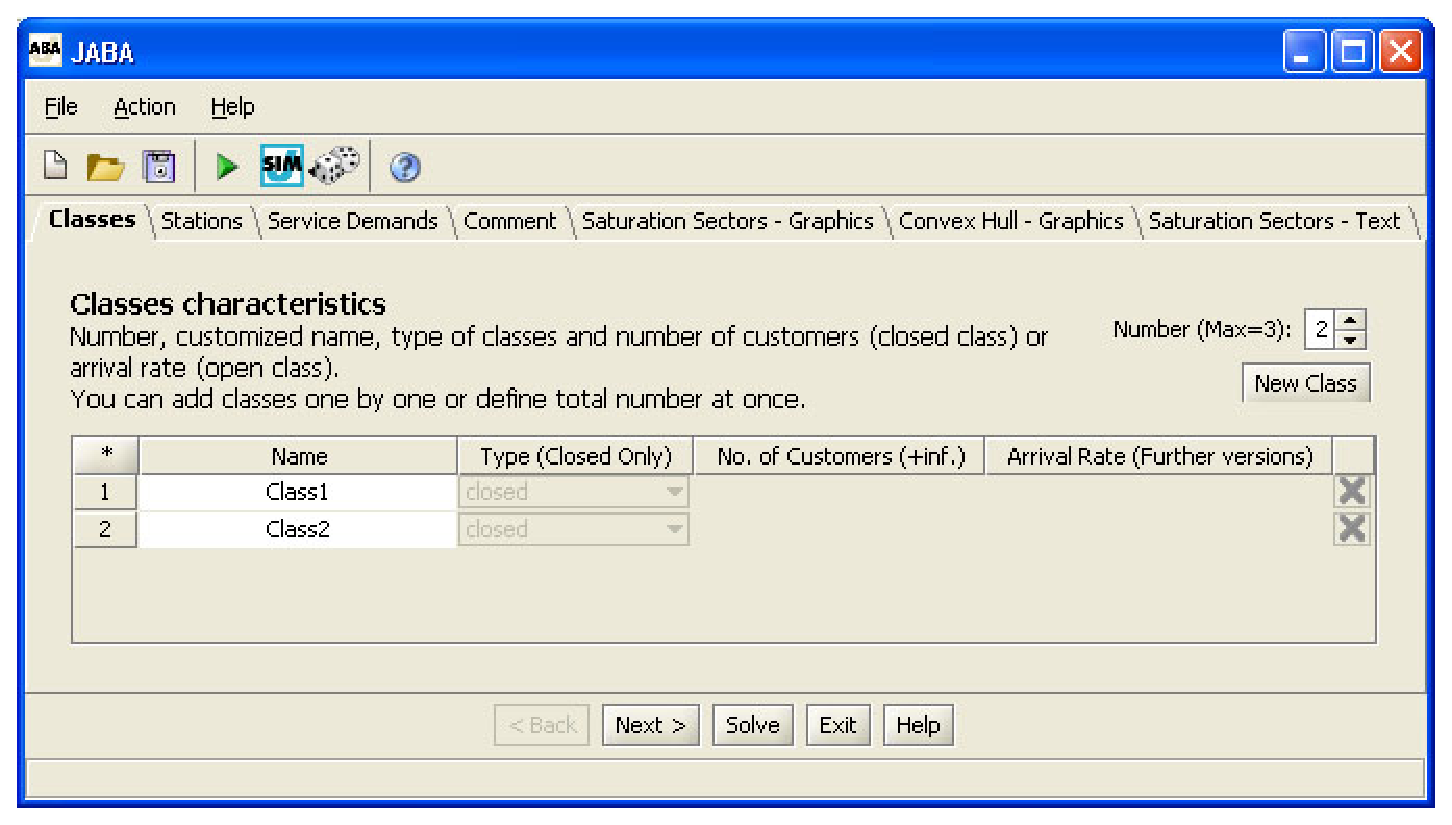
\includegraphics[scale=.5]{img/jaba/classes}
    \end{center}
    \caption{Classes tab}
    \label{fig:jaba:Classes}
\end{figure}

Three main areas are shown:
\begin{description*}
\item[Menu :] it is organized into three groups of functions. To use a
menu, click on the menu heading and choose the appropriate option.
For the description of menu entries, see \autoref{sec:jaba:Menu}
\item[Toolbar :] contains some buttons to speed up access to JABA functions
(e.g. New model, Open, Save\dots See \autoref{sec:jaba:Menu} for
details). If you move the mouse pointer over a button a tooltip will
be shown up.
\item[Page Area :] this is the core of the window. All JABA parameters are grouped in
different tabs. You can modify only a subset of them by selecting
the proper tab, as will be shown later.
\end{description*}

\section{Model definition}
Models with two or three customer classes provide estimates of wich stations are potential bottleneck.
For a brief description of basic terminology please refer to \autoref{cha:glossary}.

The workload is characterized for each station by the service
demands of every customer class.
Al least JABA works with 2 classes of custumers therefore a matrix of
service demands is required \cite{Lazowska}.

\subsection{Defining a new model}
To define a new model select toolbar button

\includegraphics[scale=.8]{img/jaba/new} or the \emph{New} command
from \emph{File} menu. The following parameters must be defined:
\begin{enumerate*}
\item \texttt{Classes}
\item \texttt{Stations} (service centers)
\item \texttt{Service demands} (or Service Times and Visits)
\item Optional short \texttt{Comment}
\end{enumerate*}

The execution of JABA produces the following graph:

\begin{itemize*}
\item Saturation Sector - Graphics
\item Convex Hull - Graphics
\end{itemize*}

\noindent And a textual report about the saturation sectors:
\begin{itemize*}
\item Saturation Sectors - Text
\end{itemize*}

\subsubsection{Input tabs}
As shown in \autoref{fig:jaba:Classes}, the parameters that
must be entered in order to define a new model are divided in four
tabs: \texttt{Classes}, \texttt{Stations}, \texttt{Service Demands}
and \texttt{Comment}.

The number of tabs become five, if you click  \emph{Service Times and
Visits} button in \texttt{Service Demands Tab}. As will be discussed
in \autoref{sec:jaba:ServiceDemand}, the \texttt{Service Demands
Tab} will be hidden and it will appear \texttt{Service Times Tab}
and \texttt{Visit Tab}. You can navigate across tabs:
\begin{itemize*}
\item using sequential wizard buttons, if enabled, at the bottom of
the window (\autoref{fig:jaba:Wizardbuttons})
\item using sequential buttons located in menu
\item using the tab selector, clicking on the corresponding
tab (\autoref{fig:jaba:Tabselector})
\end{itemize*}

\begin{figure}[htbp]
    \begin{center}
        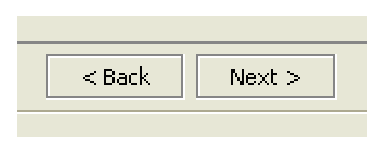
\includegraphics[scale=.5]{img/jaba/wizBut}
    \end{center}
    \caption{Wizard buttons}
    \label{fig:jaba:Wizardbuttons}
\end{figure}

\begin{figure}[htbp]
    \begin{center}
        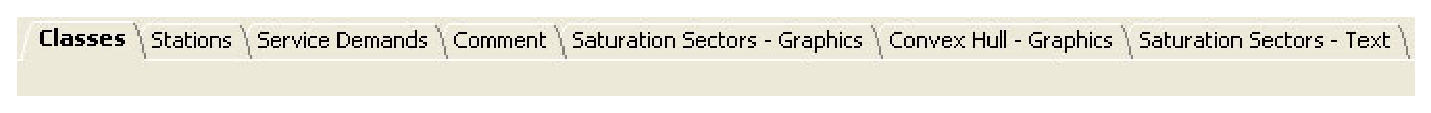
\includegraphics[scale=.5]{img/jaba/tabSel}
    \end{center}
    \caption{Tab selector}
    \label{fig:jaba:Tabselector}
\end{figure}

\subsection{Classes Tab}
An example screenshot of this tab can be seen in
\autoref{fig:jaba:Classes}. This tab allows to set the number of custumer classes.
It's possible to set two or three clesses.

The number of classes in the model can be specified in the
corresponding input area, shown in \autoref{fig:jaba:ClassNum} and
can be modified using the keyboard or the spin controls.
\begin{figure}[htbp]
    \begin{center}
        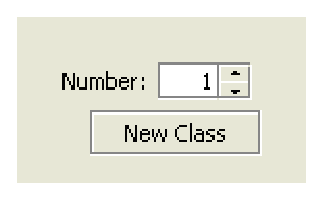
\includegraphics[scale=.5]{img/jaba/classNum}
    \end{center}
    \caption{Number of classes}
    \label{fig:jaba:ClassNum}
\end{figure}

Using the delete button
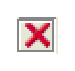
\includegraphics[scale=.6]{img/jaba/x} associated to a specific
class, a class can be removed provided that there will be at least
one class after the deletion. Similar result may be obtained using
spin controls, decreasing classes number; in this case last inserted
class will be removed.

Default class names are \emph{Class1}, \emph{Class2}, \dots
\emph{ClassN}. The model can be personalized by changing these names.

\subsection{Stations Tab}
The number of stations of the model can be specified in the
corresponding input area (\autoref{fig:jaba:stationNum}) and can be
modified using the keyboard or the spin controls.

\begin{figure}[htbp]
    \begin{center}
        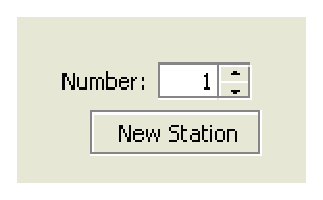
\includegraphics[scale=.5]{img/jaba/stationNum}
    \end{center}
    \caption{Number of stations}
    \label{fig:jaba:stationNum}
\end{figure}

Using the delete button
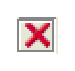
\includegraphics[scale=.6]{img/jaba/x} associated to a specific
station, a station can be removed provided that there will be at
least one station after the deletion. Similar result may be obtained decreasing stations number using spin controls; in this case last inserted station will be removed.

Default station names are \emph{Station1}, \emph{Station2}, \dots
\emph{StationN}. In order to personalize your model, you can change
and give names other than default ones.

In \autoref{fig:jaba:stations} there is only one station with
default name \emph{Station4} and there are three stations with
personalized names: \emph{CPU}, \emph{Disk1} and \emph{Disk2}.

\begin{figure}[htbp]
    \begin{center}
        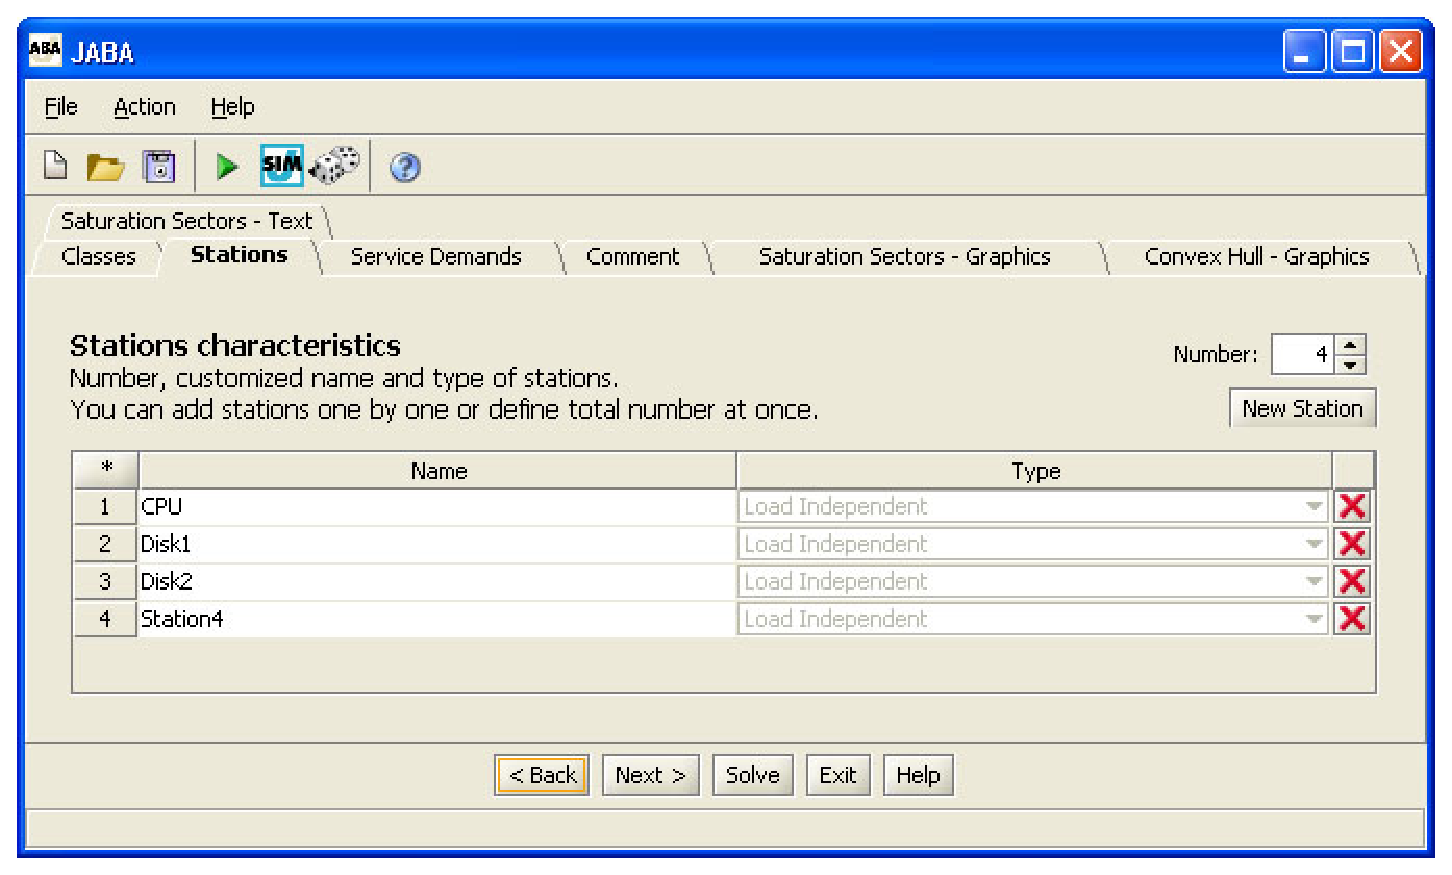
\includegraphics[scale=.5]{img/jaba/4stations}
    \end{center}
    \caption{Defining the stations name}
    \label{fig:jaba:stations}
\end{figure}


\subsection{Service Demands, Service Times and Visits Tabs}
\label{sec:jaba:ServiceDemand} Service Demands can be defined in two
ways:
\begin{itemize*}
\item directly, by entering Service Demands ($D_{kc}$)
\item indirectly, by entering Service Times ($S_{kc}$) and Visits ($V_{kc}$)
\end{itemize*}

Service demand $D_{kc}$ is the total service requirement, that is
the average amount of time that a customer of class $c$ spends in
service at station $k$ during one interaction with the system, i.e.
it's complete execution. Service time $S_{kc}$ is the average time
spent by a customer of class $c$ at station $k$ for a single visit
at that station while $V_{kc}$ is the average number of visits at
that resource for each interaction with the system.

Remember that $D_{kc} = V_{kc} * S_{kc}$ so it's simple to compute
service demands matrix starting from service times and visits
matrixes. Inverse calculation is performed with the following
algorithm:
\[
V_{kj} = \left\{
\begin{array}{ccl} 1 & \textrm{if} & D_{kc} > 0 \\
0 & \textrm{if} & D_{kc} = 0 \end{array}\right.
\]
\[
S_{kc} = \left\{ \begin{array}{ccl} D_{kc} & \textrm{if} & D_{kc}
> 0 \\ 0 & \textrm{if} & D_{kc} = 0 \end{array}\right.
\]

\subsubsection{Service Demands Tab}
In this tab you can insert directly Service Demands $D_{kc}$ for
each pair \{station~$k$-class~$c$\} in the model. \autoref{fig:jaba:ServiceDemandsTab} shown a reference screenshot can be seen: notice that a value for every $D_{kc}$ element of the $D$-matrix has already been specified because the default value assigned to newly created stations is zero.
\begin{figure}[htbp]
    \begin{center}
        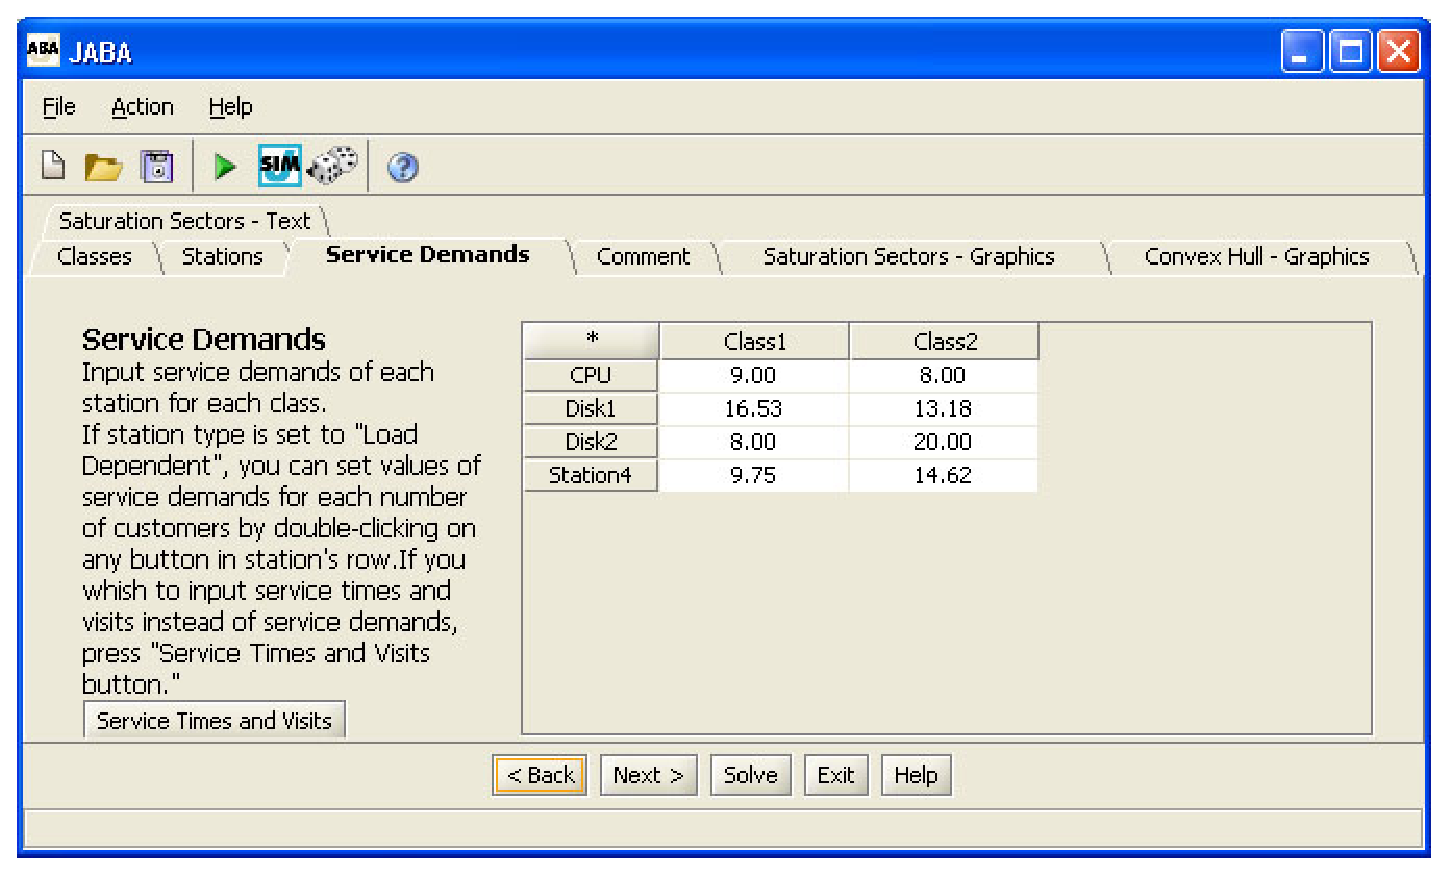
\includegraphics[scale=.5]{img/jaba/serviceDemands}
    \end{center}
    \caption{The Service Demands Tab}
    \label{fig:jaba:ServiceDemandsTab}
\end{figure}

In \autoref{fig:jaba:ServiceDemandsTab}, each job of \emph{Class1} requires an average service demand time of 6
sec to \emph{CPU}, 16.53 sec to \emph{Disk1}, 8 sec to
\emph{Disk2} and 9.75 sec to \emph{Station4}.\\

\subsubsection{Service Times and Visits Tabs}
In the former tab you can insert the Service Times $S_{kc}$ for each
pair \{station~$k$-class~$c$\} in the model, in the latter you can
enter the visits number $V_{kc}$ (See \autoref{fig:jaba:visits}).
\begin{figure}[htbp]
    \begin{center}
        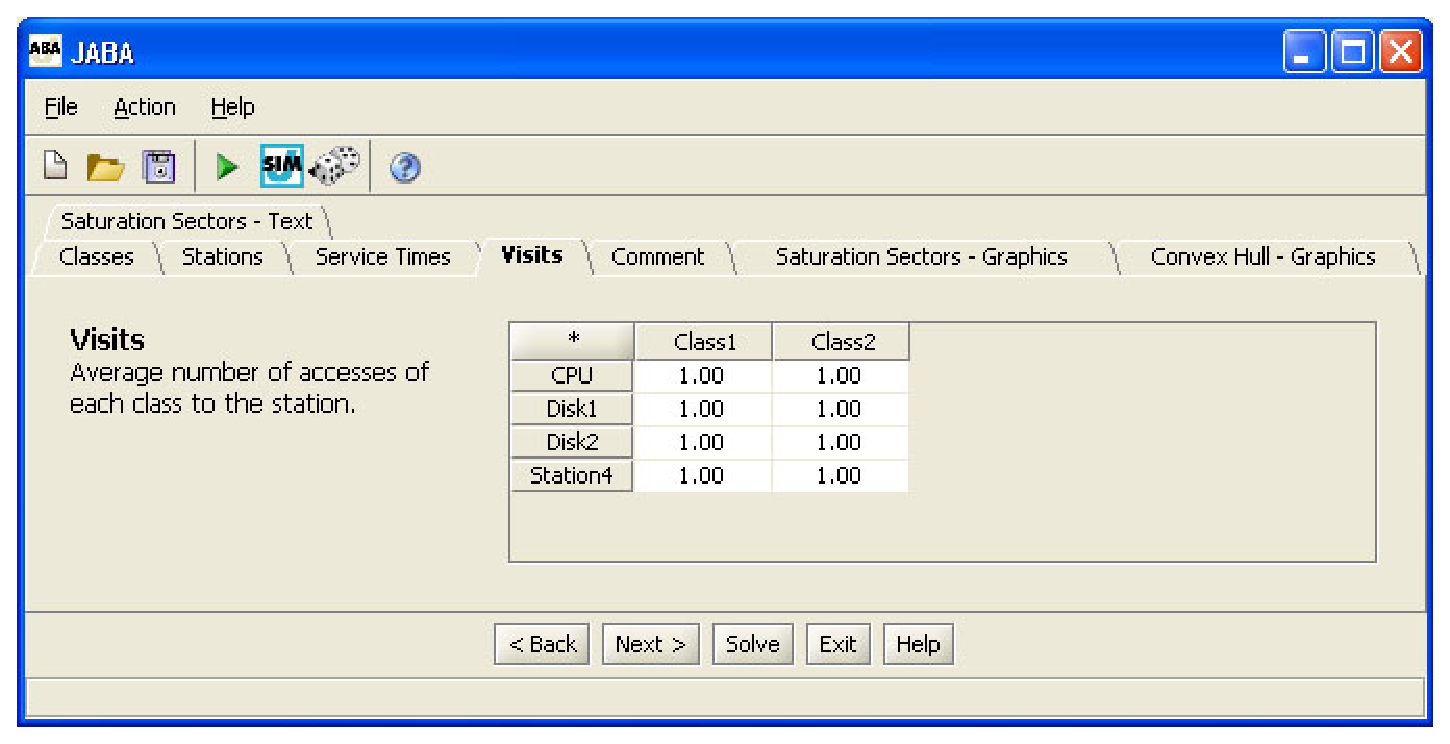
\includegraphics[scale=.5]{img/jaba/visits}
    \end{center}
    \caption{Visits Tab}
    \label{fig:jaba:visits}
\end{figure}

The layout of these tabs is similar to the one of the
\texttt{Service Demand Tab} described in the previous paragraph. The
default value for each element of the Service Times ($S$) matrix is
zero, while it's one for Visits' matrix elements.


\subsection{Comment Tab}
In this Tab, a short - optional - comment about the model can be
inserted; it will be saved with the other model parameters.


\subsection{Saturaction Sector - Graphic}
\label{sec:jaba:saturationSectorGraphic}

Using the \texttt{Solve} command the Saturaction Sector graphic appears.

\subsubsection{Two Classes graphic}

We indicate a certain mix population with the couple (N1,N2) where N1 is the percentage of the customers belong to class1 and N2 is the percentage of the customers of class2. Because the sum of N1 and N2 must be 100$\%$ we will only consider N1 (N2 can be calculated subtrahend N1 at 100). In the hypothesis that the number of customers in the system is constant (and high) it is possible to find an interval [N1 to N1'] where the same two stations are bottleneck.
We define this interval saturation sector and its extremity switching points that are the value in with the station change from non-bottleneck to bottleneck or viceversa.

It is possible to represent a saturation sector and the switching points using a bidimentional graphic \autoref{fig:jaba:saturationSector}.
\begin{figure}[htbp]
    \begin{center}
        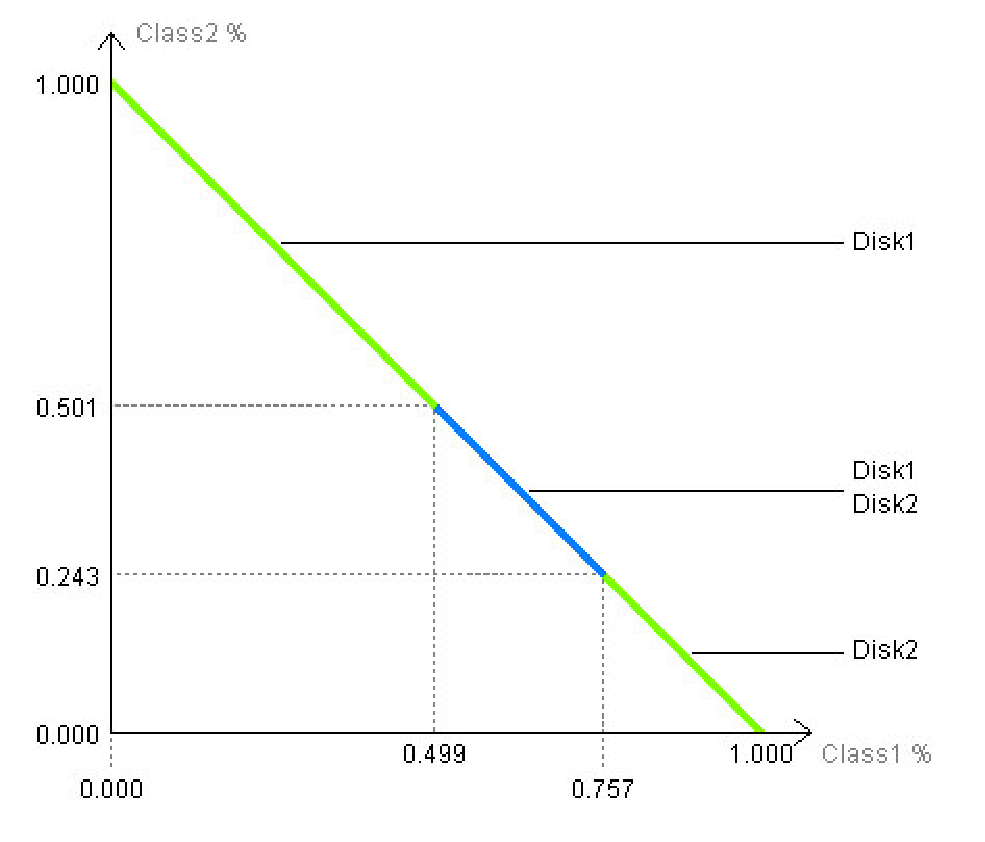
\includegraphics[scale=.5]{img/jaba/saturationSector}
    \end{center}
    \caption{Saturation Sector Graphic}
    \label{fig:jaba:saturationSector}
\end{figure}

In this example we can observe that \emph{Disk1} is a bottleneck for a mix population
among (0;1) and (0.499,0.501). At the point (0.499,0.501) color switches from green to blue because
this point is a switching point. In fact for a mix population from (0.499,0.501) to (0.757,0.243)
\emph{Disk1} and \emph{Disk2} are both bottleneck. After the point (0.757,0.243), that is a swiching
point too, only \emph{Disk2} is a bottleneck.


\subsubsection{Three Classes graphic}

Suppose we can split the customers of our system in 3 class of customers, a specific population mix could be represented by a point whose coordinates are the percentage of customers of a specific class.
on a triangle that has the vertex in the points (1,0,0), (0,1,0) e (0,0,1). The triangle area represent every possible population mix. So we can divide the triangle in different sub-areas and each area
rapresent a population mix range where one, two or more stations are bottleneck at the same time.
It is clearly understandable that we have no more a switching point (such as in the two classes graph)
but a switching segment.
\begin{figure}[htbp]
    \begin{center}
        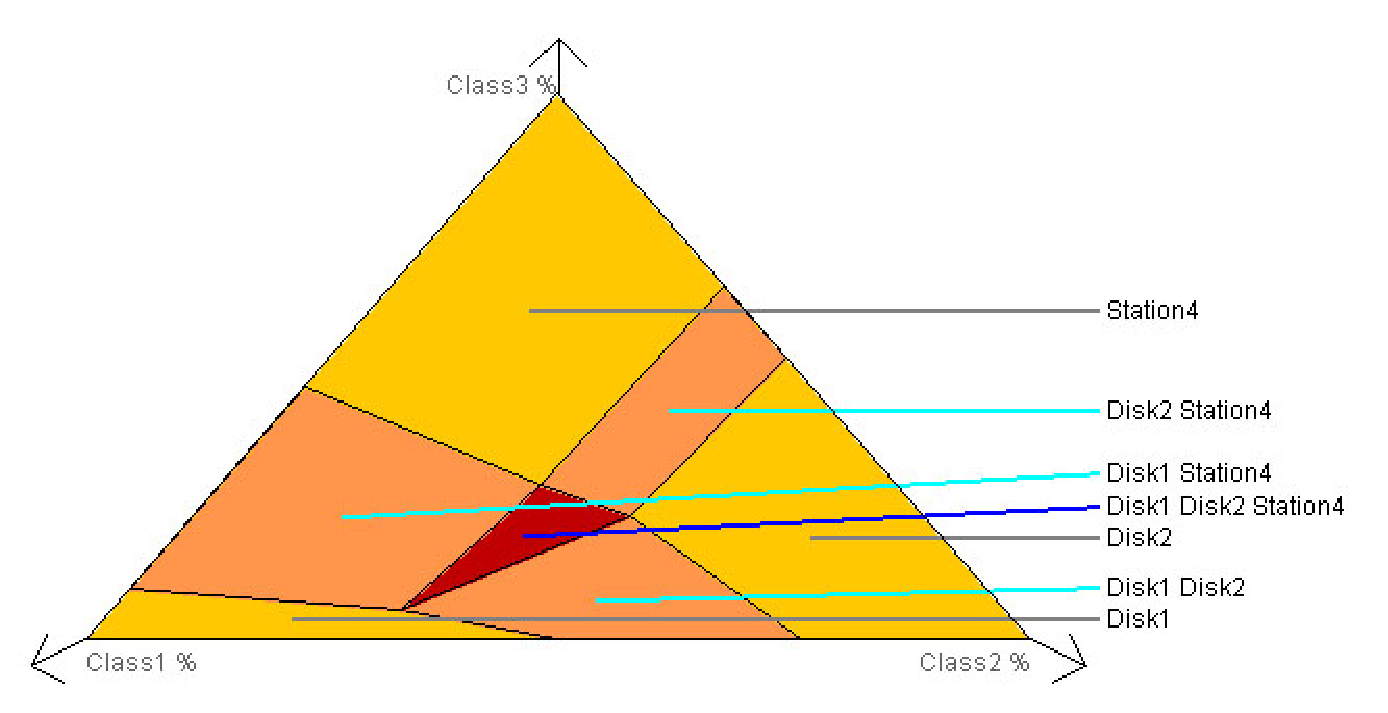
\includegraphics[scale=.5]{img/jaba/saturationSector3Class}
    \end{center}
    \caption{Saturation Sector Graphic}
    \label{fig:jaba:saturationSector3Class}
\end{figure}

In this example \autoref{fig:jaba:saturationSector3Class} we can observe a big area,on the top of the triangle, that rapresents the range of mix population where \emph{Station4} is a bottleneck. In the center of the triangle there is a little red area that rapresent the range of mix population where \emph{Disk1}, \emph{Disk2} and \emph{Station4} are all bottleneck.

This graph is useful for understanding what station begin bottlenek and when but it is not simple to recornize the exat value of the swiching segment. In order to obtain the exact value select the ``Saturation Sector - Text'' tab \autoref{sec:jaba:saturationSectorText}.



\subsection{Convex Hull - Graphic}
\label{sec:jaba:convexHullGraphic}

Using the \texttt{Solve} command and selecting the ``Convex Hull - Graphic''
tab the Convex Hull graphic is show.

\subsubsection{Overview}
The Convex Hull graphic implements the polyhedral analysis technique.
The polyhedral analysis technique implemented in JABA is limited to queueing networks with customers grouped in two classes. The points in the graph are obtained from the service demand matrix as follows. Each station corresponds to a point on the graph whose co-ordinates are represented by the service demand of the two customer classes. For example, a queue with service demands 10 sec for class 1, and 15 sec for class 2 is represented as a point with coordinates (10,15).  Then JABA builds the convex hull of this set of points, that is the smallest convex set containing all the points.

The distinction of queues among the different types of bottleneck and non-bottleneck classes can be immediately operated from the knowledge of the convex hull using the following rules:
\begin{itemize*}
    \item All \emph{potential bottlenecks} lie on the boundary of the convex polytope.
    \item All \emph{dominated} station are interior points P of the convex polytope such that there is at least one point Q whose co-ordinates are all higher or equal in value than those of P;
    \item All non-dominated stations in the interior of the convex polytope are \emph{masked-off} stations.
The application of these rules is described below in the case study.
\end{itemize*}
\begin{figure}[htbp]
    \begin{center}
        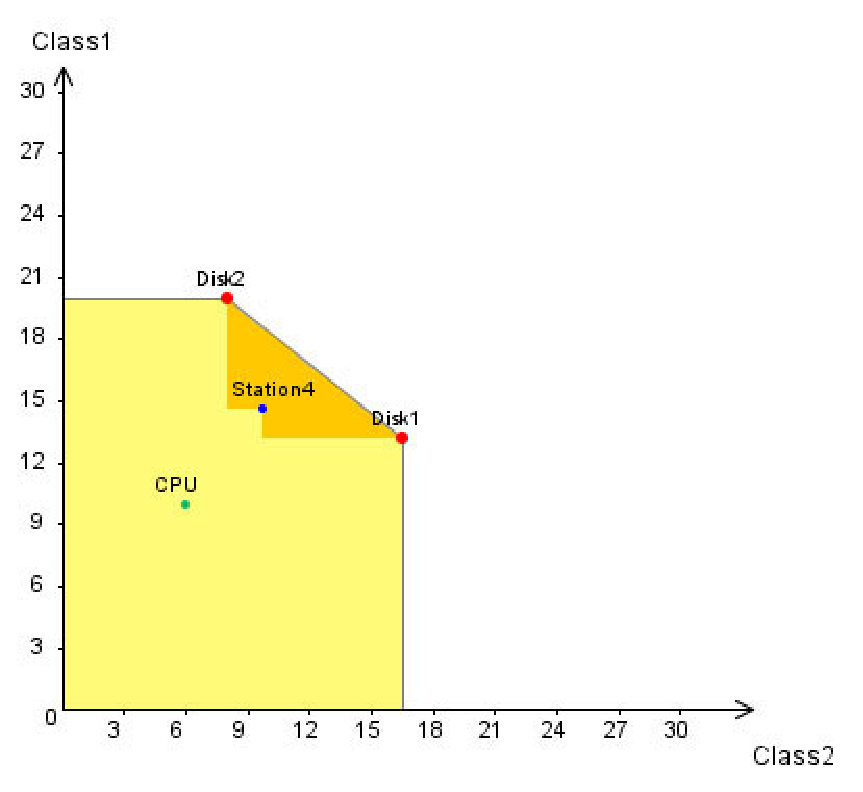
\includegraphics[scale=.5]{img/jaba/convexHull}
    \end{center}
    \caption{Convex Hull Graphic}
    \label{fig:jaba:convexHull}
\end{figure}

>From this plot,\autoref{fig:jaba:convexHull} we can see that \emph{Disk1} and \emph{Disk2} (depicted in red) lie on the boundary of the convex hull, thus are potential bottlenecks. \emph{CPU} (green) is instead a dominated non-bottleneck station, since  it is dominated by \emph{Sation4} and \emph{Disk1}. \emph{Sation4} (blue) is also in the interior of the convex hull, but it is a non-bottleneck station as there is no other point with all coordinates greater than those of \emph{Sation4} so it is a masked-off station.

\subsubsection{Determining points coordinates}

In order to gain exact information about the coordinates of a point it is sufficient to click, using the left button of the mouse, on the point and additional information will appear after the point's name. If the clicked point is a dominated one, then it will be possible to see by which point (there could be more than one) it is dominated.
\begin{figure}[htbp]
    \begin{center}
        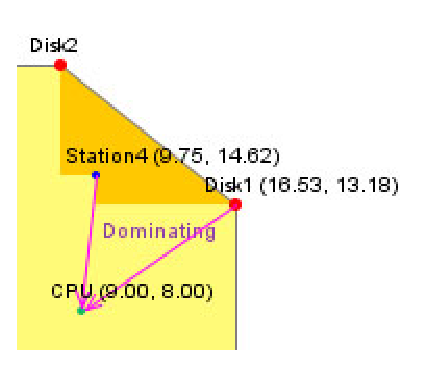
\includegraphics[scale=.8]{img/jaba/convexHullCoordinate}
    \end{center}
    \caption{Convex Hull Graphic while CPU is selected}
    \label{fig:jaba:convexHullCoordinate}
\end{figure}

\subsubsection{Determining heavy-load throughputs and bottlenecks under a certain workload mix}

Clicking (left button) on the line that it connects two bottleneck stations you can obtain information about the saturation sector  such as the interval of mix population that make possible the bottleneck and also the throughput of the two classes.
\begin{figure}[htbp]
    \begin{center}
        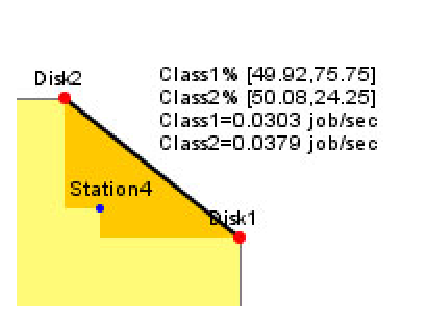
\includegraphics[scale=.8]{img/jaba/convexHullSaturationSector}
    \end{center}
    \caption{Convex Hull Graphic while saturation sector is selected}
    \label{fig:jaba:convexHullSaturationSector}
\end{figure}

\subsubsection{Move a station to another point}
\label{sec:jaba:convexHullDrag}
Now suppose  that we have to analyze the upgrade of the station \emph{Station4}, the new \emph{Station4} will have half demand for both the customer's classes compared to the old one. In order to do this we can change the value in the demand's table of JABA or click on the point (left button) and drag it in the new position.
\begin{figure}[htbp]
    \begin{center}
        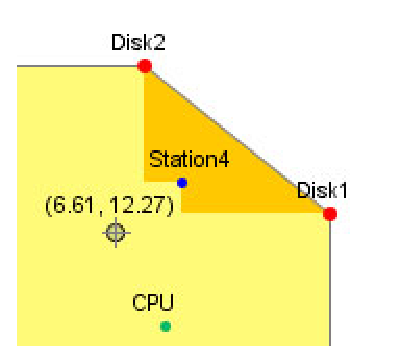
\includegraphics[scale=.7]{img/jaba/convexHullDragPoint}
    \end{center}
    \caption{Convex Hull Graphic while is dragging a point}
    \label{fig:jaba:convexHullDragPoint}
\end{figure}

While dragging the point temporary co-ordinates are shown and when the point is released all data are update and a new graph is created.

\subsubsection{Identify a point's label in a crowded area}
It is possible that a area of the graph could be crowded of points whose names are difficult to read as showed in  thefollowing graph \autoref{fig:jaba:convexHullaCrowded}.
\begin{figure}[htbp]
    \begin{center}
        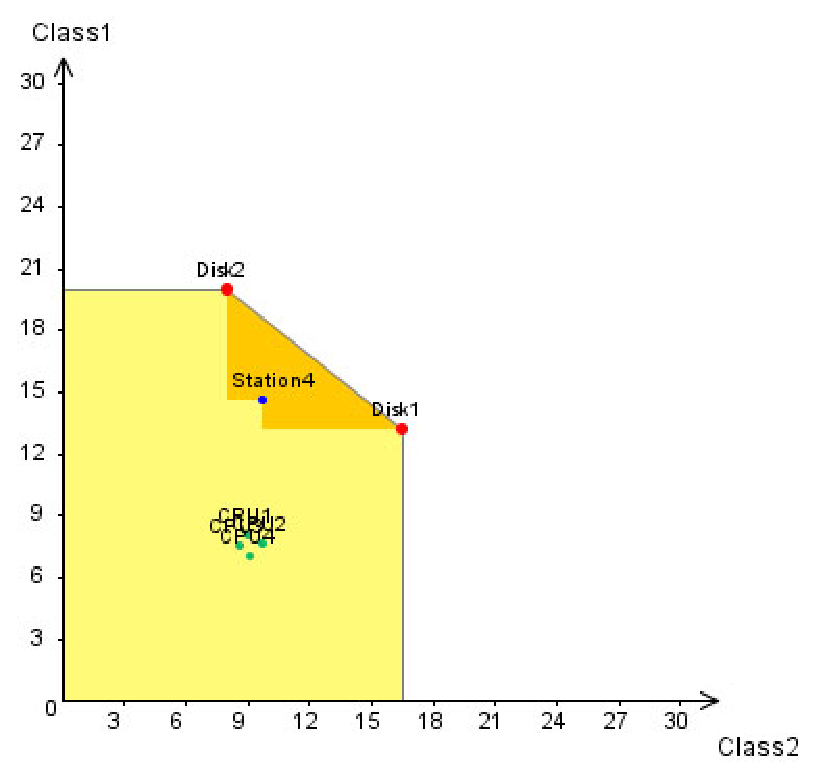
\includegraphics[scale=.5]{img/jaba/convexHullCrowded}
    \end{center}
    \caption{Convex Hull Graphic whith a crowded area}
    \label{fig:jaba:convexHullaCrowded}
\end{figure}

It is difficult to understand - or simply read - which of the dominated point the label belongs to; at first we can try to change the zoom, we can therefore zooming in by a double click on the mouse's left button or zooming out by a double click on the mouse's right button.
If the zooming is no enough we can try filtering the zone and freeing only some points. In order to filter the area is enough to select it keeping the mouse's left button pressed. The background of the selected area will become grey, points will become dark grey and their labels will disappear.
\begin{figure}[htbp]
    \begin{center}
        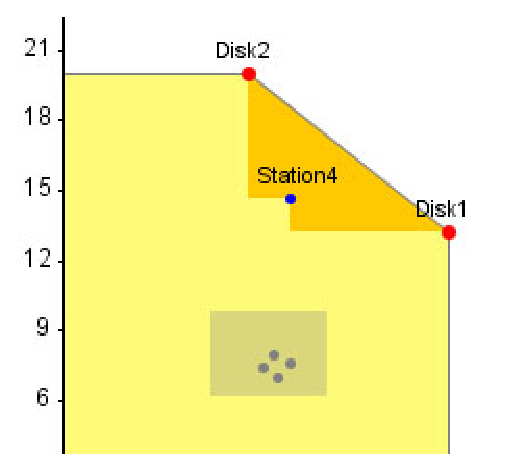
\includegraphics[scale=.5]{img/jaba/convexHullFiltered}
    \end{center}
    \caption{Convex Hull Graphic whith a filtered area}
    \label{fig:jaba:convexHullaFiltered}
\end{figure}

Now we try to reduce the filtered area adding some free area; to do that we select the area that we wish to free keeping the mouse's right button pressed. In the following example we have set the tallest point free.
\begin{figure}[htbp]
    \begin{center}
        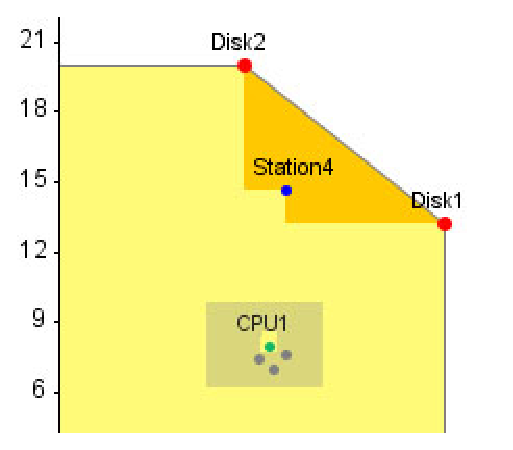
\includegraphics[scale=.5]{img/jaba/convexHullFree}
    \end{center}
    \caption{Convex Hull Graphic whith a filtered area}
    \label{fig:jaba:convexHullaFree}
\end{figure}

Only the name of the station that is in the free area is showed.


\subsection{Saturation Sector - Text}
\label{sec:jaba:saturationSectorText}
It's a simple report about the saturation sector, for each saturation sector you can find:
\begin{itemize*}
\item The station that are bottleneck
\item The switching point or the switching segment bound points.
\end{itemize*}
This tab could be helpful in the Saturation Sector graphic of three classes of costumers.\autoref{sec:jaba:saturationSectorGraphic}



\subsection{Modification of a model}
To modify system parameters return to the main window and enter new
data or moving a station in Convex Hull - graphic tab (see \autoref{sec:jaba:convexHullGraphic}).
After the modifications, if you use \texttt{Solve} command, the
new graphs will show. You can \texttt{save} this
new model with the previous name - overwriting the previous one - or
\texttt{save} it with a different name or in a different directory.

\section{Menu entries}
\label{sec:jaba:Menu}
\subsection{File}
\subsubsection{New}
Use this command in order to create a new JABA model.

\noindent
\begin{tabular}{ll}
Shortcut on Toolbar: & 
\includegraphics[scale=.8]{img/jaba/new}\\
Accelerator Key: & CTRL+N
\end{tabular}

\subsubsection{Open}
Use this command to open an existing model. You can only open one
model at time, to edit two or more models start more than one
instance of JABA. If current model was modified since its creation
or last save action, a popup window will be shown for confirmation.

It's possible to open not only models saved with JABA (*.jaba), but
also with other programs of the suite (for example JMVA *.jmva, JSIM
*.jsim and JMODEL *.jmodel). Whenever a foreign data file is opened, a
conversion is performed and error/warnings occurred during
conversion will be reported in a window.

Models are stored in XML format, see \emph{JMT system manual} for a
detailed description.

\noindent
\begin{tabular}{ll}
Shortcut on Toolbar: & 
\includegraphics[scale=.8]{img/jaba/open}\\
Accelerator Key: & CTRL+O
\end{tabular}

\subsubsection{Save}
Use this command in order to save the active document with its
current name in the selected directory.

When you save a document for the first time, JABA displays the Save
As dialog box so you can rename your document. If you save a model
after its resolution, results are stored with model definition data.

\noindent
\begin{tabular}{ll}
Shortcut on Toolbar: & 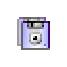
\includegraphics[scale=.8]{img/jaba/save}\\
Accelerator Key: & CTRL+S
\end{tabular}

\subsubsection{Exit}
Use this command in order to end a JABA session. You can also use
the Close command on the application Control menu. If current model
was modified since its creation or last save action, a popup window
will be shown for confirmation.

\noindent
\begin{tabular}{ll}
\\
Accelerator Key: & CTRL+Q
\end{tabular}

\subsection{Action}
\subsubsection{Solve}
Use this command when model description is terminated and you want
to start the solution of the model. At the end of the process the
Saturation Sector - Graphic \autoref{sec:jaba:saturationSectorGraphic} will show.

\noindent
\begin{tabular}{ll}
Shortcut on Toolbar: & 
\includegraphics[scale=.8]{img/jaba/solve}\\
Accelerator Key: & CTRL+L
\end{tabular}

\subsubsection{Randomize}
Use this command in order to insert random values into Service
Demands - or Service Times - table.

\noindent
\begin{tabular}{ll}
Shortcut on Toolbar: & 
\includegraphics[scale=.8]{img/jaba/randomize}\\
Accelerator Key: & CTRL+R
\end{tabular}


\subsection{Help}
\subsubsection{JABA Help}
Not still avaiable.

\section{Examples}
In this section we will describe some examples of model
parametrization and solution using JABA exact solver. Step-by-step
instructions are provided in two examples:
\begin{enumerate*}
\item A two class model
(\autoref{sec:jaba:example1})
\item A three class model
(\autoref{sec:jaba:example2})
\end{enumerate*}

\subsection{Example 1 - A two class model}
\label{sec:jaba:example1} Solve the two class model specified in
\autoref{fig:jaba:Example1topology}.
\begin{figure}[htbp]
    \begin{center}
        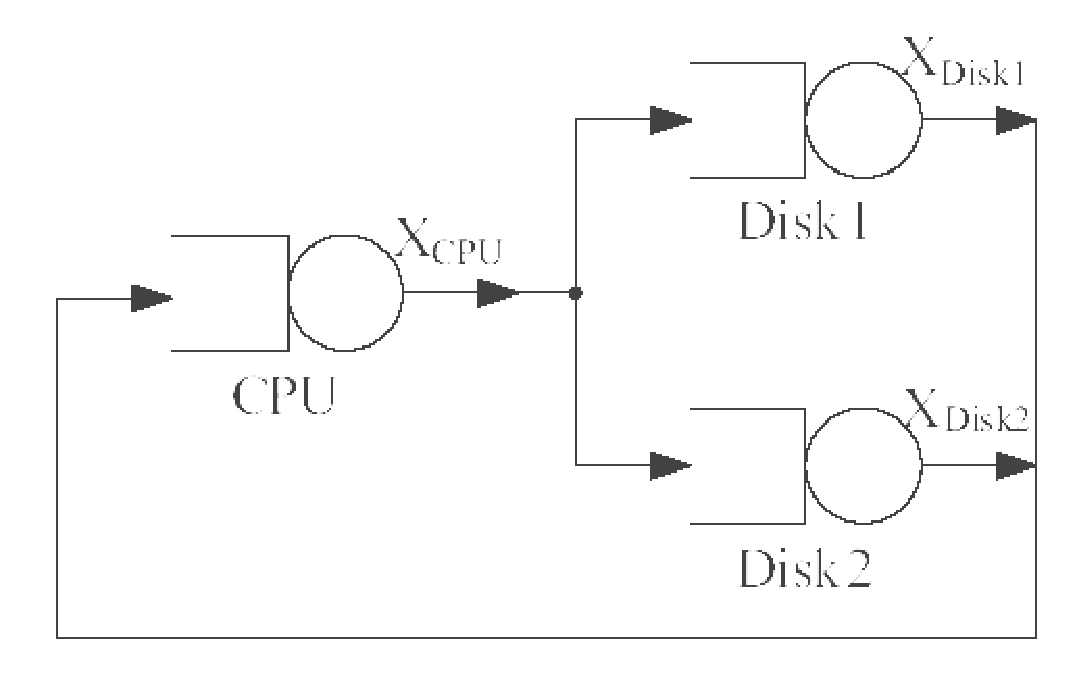
\includegraphics[scale=.35]{img/jaba/example1}
    \end{center}
    \caption{Example 1 - network topology}
    \label{fig:jaba:Example1topology}
\end{figure}

There are three stations (named
\emph{CPU}, \emph{Disk1} and \emph{Disk2}).
Service demands for each station are reported in
\autoref{tab:jaba:example1ServDemand}.

\begin{table}[htbp]
\begin{center}
\begin{tabular}{c|r|r|r|}
& \multicolumn{1}{c|}{CPU} & \multicolumn{1}{c|}{Disk1} & \multicolumn{1}{c|}{Disk2} \\
\hline
FirstClass & $2.60$ & $7.02$ & $4.81$ \\
SecondClass & $7.02$ & $4.51$ & $5.70$ \\
\hline
\end{tabular}
\end{center}
\caption{Example 1 - service demand}
\label{tab:jaba:example1ServDemand}
\end{table}

\subsubsection{Step 1 - Classes Tab}
\begin{itemize*}
\item use New command to create a new JABA document
\item by default, you have already two classes
\item if you like, substitute default \emph{Class1} and \emph{Class2} name with a customized
one (\emph{FirstClass} and \emph{SecondClass} in our example)
\end{itemize*}

At the end of this step, the \texttt{Classes Tab} should look like
\autoref{fig:jaba:example1Classes}.

\begin{figure}[htbp]
    \begin{center}
        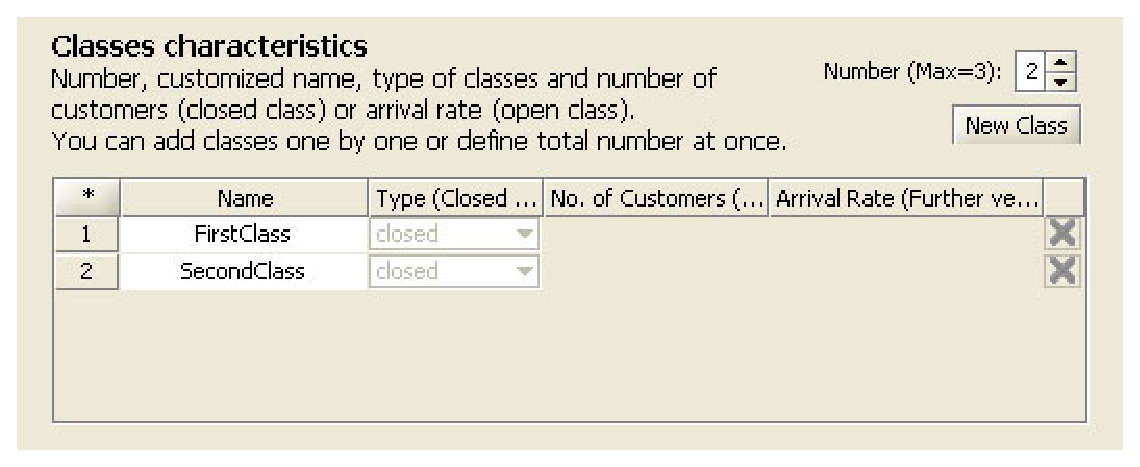
\includegraphics[scale=.7]{img/jaba/example1Class}
    \end{center}
    \caption{Example 1 - input data (Classes Tab)}
    \label{fig:jaba:example1Classes}
\end{figure}

\subsubsection{Step 2 - Stations Tab}
\begin{itemize*}
\item use \texttt{Next $>$} command to switch to \texttt{Stations Tab}
\item digit number 3 into stations number textbox or select number
3 using spin controls or push \emph{New Station} button twice.
Now your model has three stations with a default name
\item if you want you can change station names. Substitute \emph{CPU} for
default name \emph{Station1}, substitute \emph{Disk1} for default
name \emph{Station2}, substitute \emph{Disk2} for default name
\emph{Station3}
\end{itemize*}

At the end of this step, the \texttt{Stations Tab} should look like
\autoref{fig:jaba:example1Stations}.

\begin{figure}[htbp]
    \begin{center}
        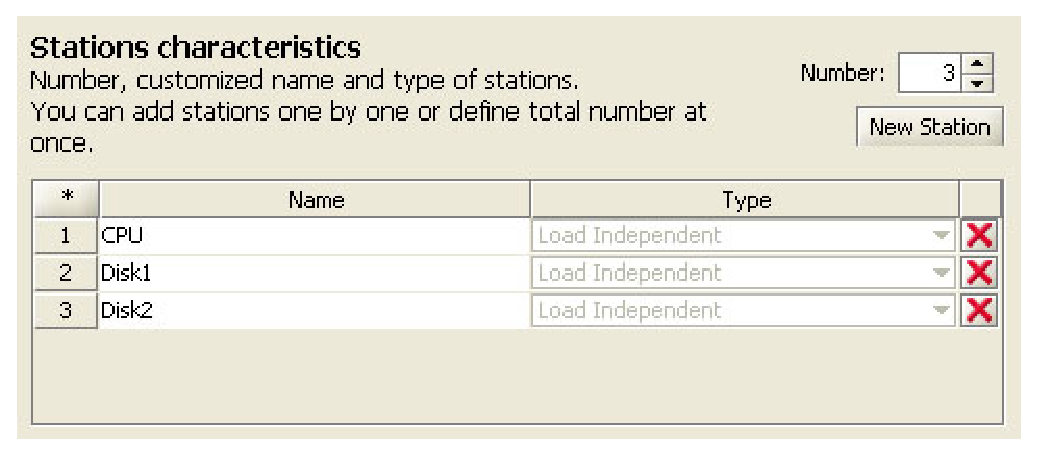
\includegraphics[scale=.7]{img/jaba/example1Stations}
    \end{center}
    \caption{Example 1 - input data (Stations Tab)}
    \label{fig:jaba:example1Stations}
\end{figure}

\subsubsection{Step 3 - Service Demand Tabs}
\begin{itemize*}
\item use \texttt{Next $>$} command to switch to \texttt{Service Demands Tab}
\item you can input all Demands in the table.
\item press \emph{Service Time and Visit} button if you don't know
the Service Demands of the three stations. After button pressure,
the \texttt{Service Demands Tab} will be hidden and \texttt{Service
times Tab} and \texttt{Visit Tab} will appear. Now Service
Times and number of Visits should be typed.
\end{itemize*}

At this point, the \texttt{Service Demands Tab} should look like
\autoref{fig:jaba:example1ServiceDemand}.

\begin{figure}[htbp]
    \begin{center}
        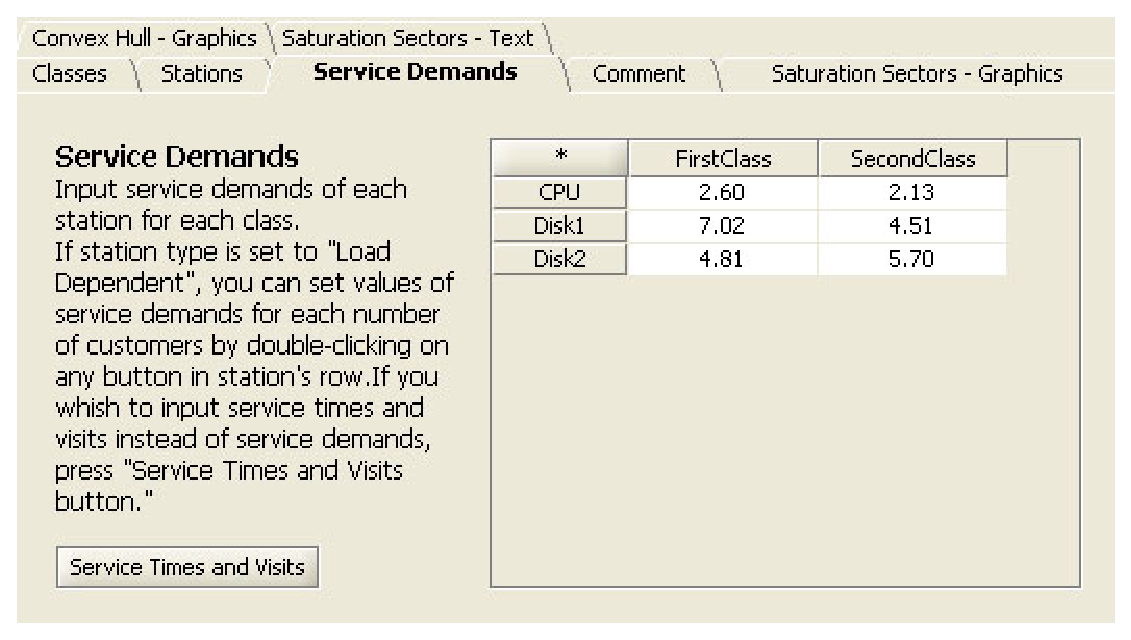
\includegraphics[scale=.75]{img/jaba/example1ServiceDemand}
    \end{center}
    \caption{Example 1 - input data (Service Demand Tab)}
    \label{fig:jaba:example1ServiceDemand}
\end{figure}


\subsubsection{Step 4 - Saturation Sectors - Graphics}


Use \texttt{Solve} command to start the solution of input model.
In the \textit{Saturation Sector - Grlaphic Tab} will be displayed a graphic like the one of
\autoref{fig:jaba:example1SatSector}.

\begin{figure}[htbp]
    \begin{center}
        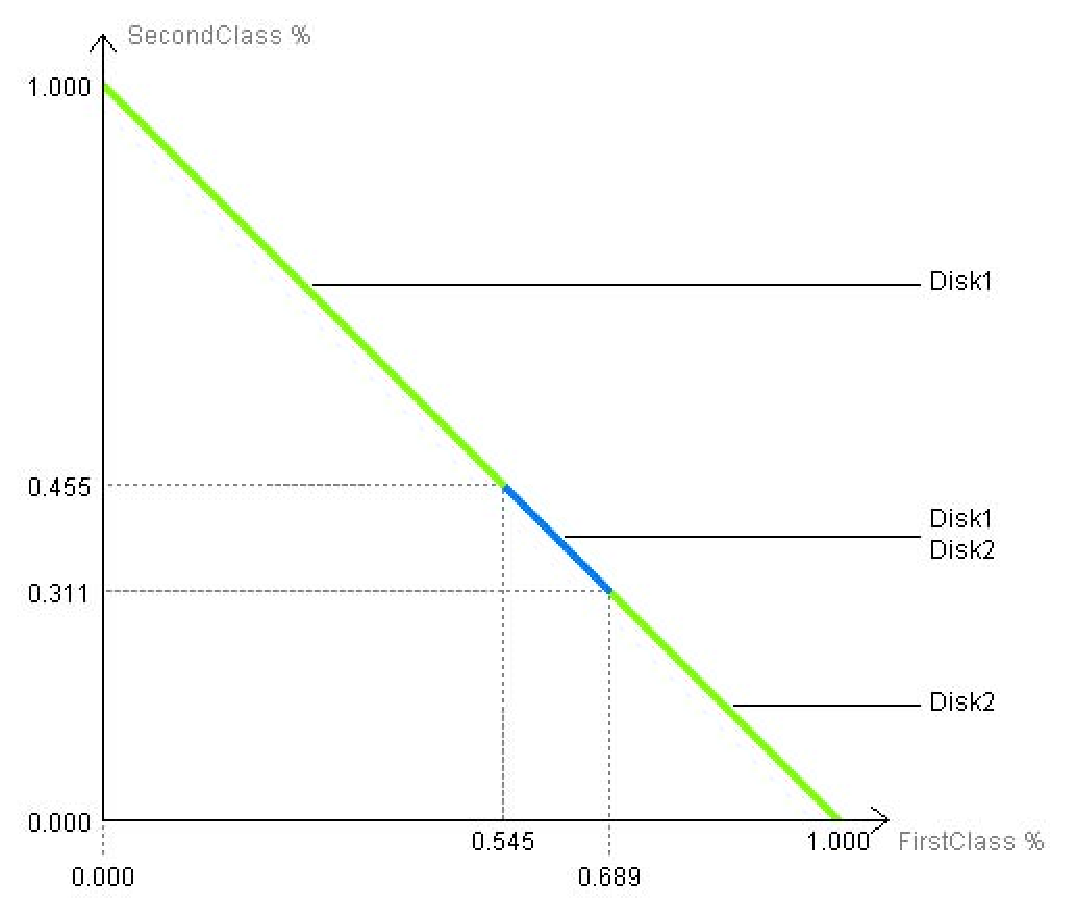
\includegraphics[scale=.5]{img/jaba/example1SatSector}
    \end{center}
    \caption{Example 1 - Saturation Sectors Graphics}
    \label{fig:jaba:example1SatSector}
\end{figure}

This graphic show the range of mix population where two or more stations are both bottleneck.
In this example \textit{Disk1} and \textit{Disk2} are both bottleneck when \textit{FirstClass} is among
\textit{0.545 - 0.689} and \textit{SecondClass} is among \textit{0.311 - 0.455}

\subsubsection{Step 5 - Convex Hull - Graphics}
Using \texttt{Next $>$} command to switch to \texttt{Convex Hull - Graphics} and a graphic like \autoref{fig:jaba:example1ConvexHull} will be shown.

\begin{figure}[htbp]
    \begin{center}
        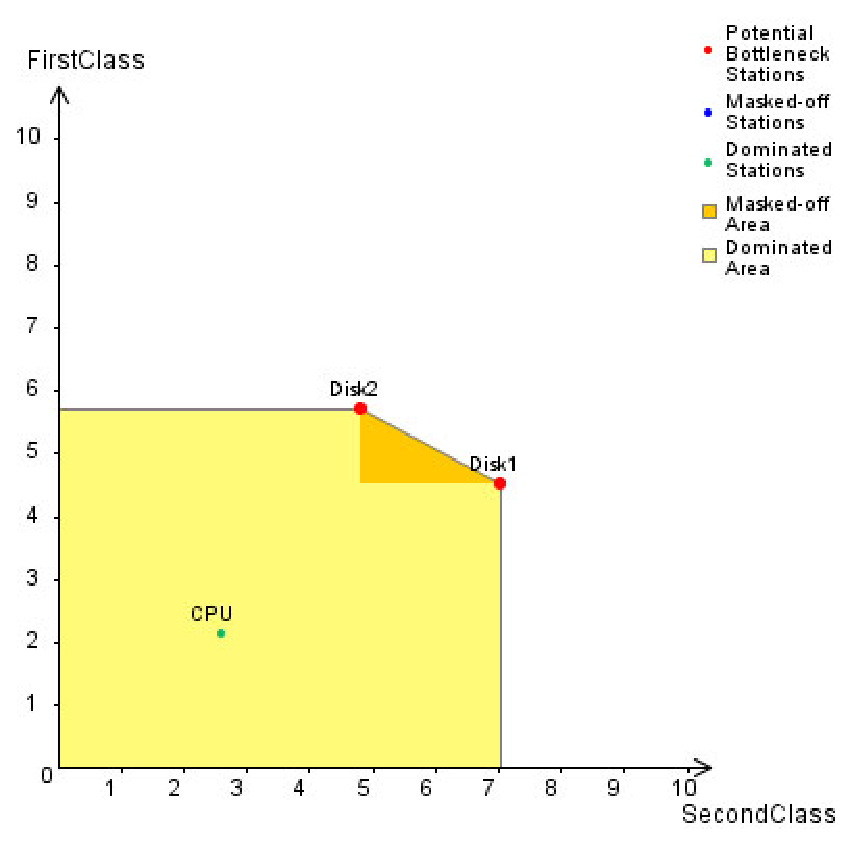
\includegraphics[scale=.6]{img/jaba/example1ConvexHull}
    \end{center}
    \caption{Example 1 - Convex Hull - Graphics}
    \label{fig:jaba:example1ConvexHull}
\end{figure}

This graphic implements the polyhedra analysis technique. The points on this graphic represent the stations. Dominated stations are green, masked-off ones are blue and bottlenek ones are red. If you click on a station, additional information will be shown, otherwise you can drag a station and see what will change in your model.

\subsubsection{Step 6 - Saturation Sectors - Text}

If you use \texttt{Next $>$} command again you will see the \textit{Saturation Sectors - Text}, a simple textual report about the Saturation Sectors.


\subsection{Example 2 - A three class model}
\label{sec:jaba:example2} Solve the multiclass open model specified
in \autoref{fig:jaba:Example2topology}.
\begin{figure}[htbp]
    \begin{center}
        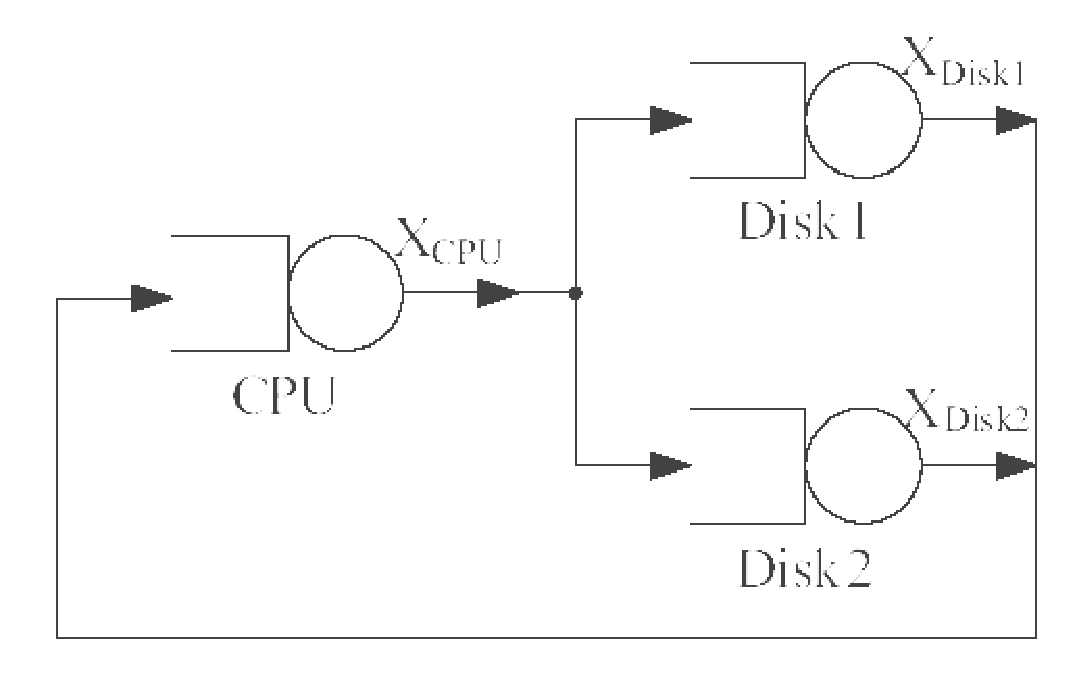
\includegraphics[scale=.35]{img/jaba/example2}
    \end{center}
    \caption{Example 2 - network topology}
    \label{fig:jaba:Example2topology}
\end{figure}
The model is characterized by three $A$ , $B$ and $C$.
There are three
stations, identified with names \emph{CPU},
\emph{Disk1} and \emph{Disk2}. Service times and visits for stations
are shown in \autoref{tab:jaba:example2ServTimes} and \autoref{tab:jaba:example2Visits}.

\begin{table}[htbp]
\begin{center}
\begin{tabular}{c|r|r|r|r|r|}
& \multicolumn{1}{c|}{CPU} & \multicolumn{1}{c|}{Disk1} & \multicolumn{1}{c|}{Disk2} \\
\hline
Class $A$ [s]& $0.01$ & $0.38$ & $0.30$ \\
Class $B$ [s]& $0.02$ & $0.62$ & $0.80$ \\
Class $C$ [s]& $0.09$ & $0.42$ & $0.50$ \\
\hline
\end{tabular}
\end{center}
\caption{Example 2 - service times}
\label{tab:jaba:example2ServTimes}
\end{table}

\begin{table}[htbp]
\begin{center}
\begin{tabular}{c|r|r|r|r|r|}
& \multicolumn{1}{c|}{CPU} & \multicolumn{1}{c|}{Disk1} & \multicolumn{1}{c|}{Disk2} \\
\hline
Class $A$ & $101.0$ & $60.0$ & $40.0$ \\
Class $B$ & $44.0$ & $16.0$ & $27.0$ \\
Class $C$ & $63.0$ & $21.0$ & $35.0$ \\
\hline
\end{tabular}
\end{center}
\caption{Example 2 - number of visits}
\label{tab:jaba:example2Visits}
\end{table}


\subsubsection{Step 1 - Classes Tab}
It is the same procedure of the Example 1 (\autoref{sec:jaba:example1}). You have only to add one more class.
\subsubsection{Step 2 - Stations Tab}
It is the same procedure of the Example 1 (\autoref{sec:jaba:example1}).
\subsubsection{Step 3 - Service Times and Visits Tabs}
\begin{itemize*}
\item use \texttt{Next $>$} command to switch to \texttt{Service Demands Tab}
\item press \emph{Service Time and Visit} button if you don't know
the Service Demands of the three stations, Now Service
Times and number of Visits should be typed. After button pressure,
the \texttt{Service Demands Tab} will be hidden and \texttt{Service
times Tab} and \texttt{Visit Tab} will appear
\item you can input all Service Times in the table.
\end{itemize*}

At this point, the \texttt{Service Times Tab} should look like
\autoref{fig:jaba:example2Service}.

\begin{figure}[htbp]
    \begin{center}
        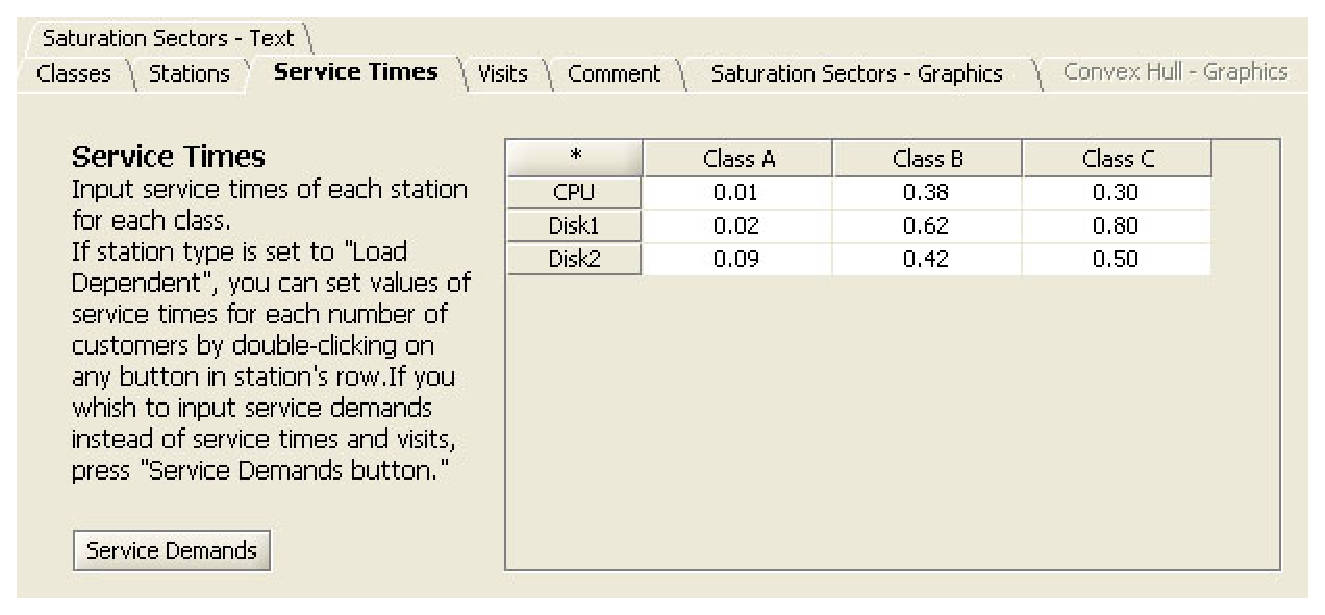
\includegraphics[scale=.70]{img/jaba/example2Service}
    \end{center}
    \caption{Example 2 - input data (Service Times Tab)}
    \label{fig:jaba:example2Service}
\end{figure}

\begin{itemize*}
\item use \texttt{Next $>$} command to switch to \texttt{Visits Tab}
\item input number of visits for each center in the
table.
\end{itemize*}

At the end of this step, the \texttt{Visits Tab} looks like
\autoref{fig:jaba:example2Visits}.

\begin{figure}[htbp]
    \begin{center}
        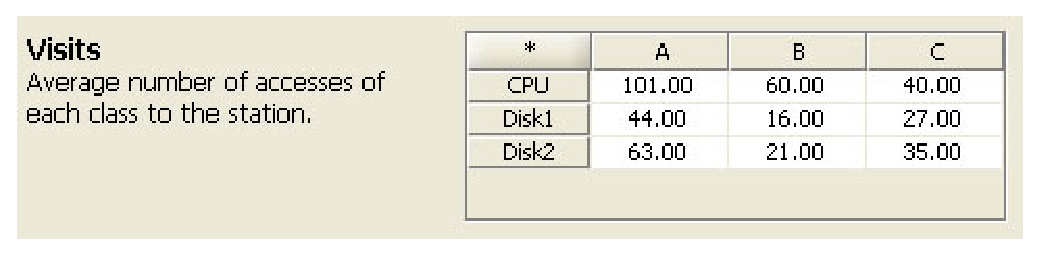
\includegraphics[scale=.8]{img/jaba/example2Visits}
    \end{center}
    \caption{Example 2 - input data (Visits Tab)}
    \label{fig:jaba:example2Visits}
\end{figure}


\subsubsection{Step 4 - Saturation Sectors - Graphics}


Use \texttt{Solve} command to start the solution of the input model.
In the \textit{Saturation Sector - Graphic Tab} will be displayed a graphic like the one of
\autoref{fig:jaba:example2SatSector}.

\begin{figure}[htbp]
    \begin{center}
        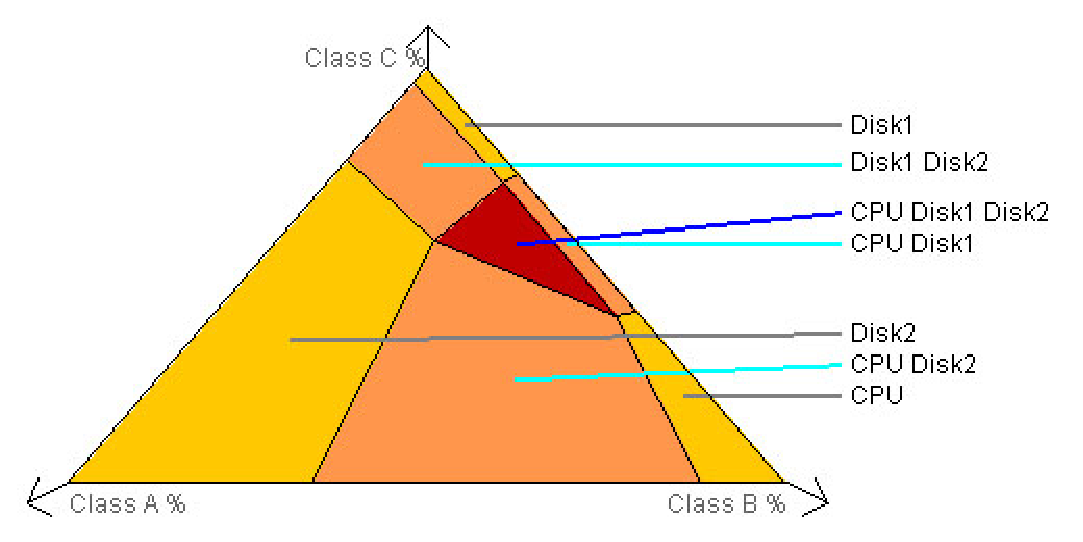
\includegraphics[scale=.75]{img/jaba/example2SatSector}
    \end{center}
    \caption{Example 2 - Saturation Sectors Graphics}
    \label{fig:jaba:example2SatSector}
\end{figure}

This graphic show the range of mix population where two or more stations are both bottleneck.
For example the orange area is a renge of mix population in which \textit{Disk1} and \textit{Disk2} are both bottlenek.

\subsubsection{Step 5 - Saturation Sectors - Text}

If you use \texttt{Next $>$} command again you will see the
\textit{Saturation Sectors - Text}, a simple textual report about
the Saturation Sectors.
